\chapter{Berechnug zu den Kräften der Halterung}\label{sec:halterkraefte}
Abbildungen \ref{abb_AnhangHK1} bis \ref{abb_AnhangHK3} zeigen die Kräfte am Grid Fin und den Halterungen, wie sie in Abschnitt \ref{sec:AktuSim} beschrieben wurden, aus unterschiedlichen Perspektiven. Zunächst werden die Kräfte- und Momentengleichgewichte aufgestellt und dann daraus die einzelnen Kräfte in den Halterungen in Abhängigkeit der aerodynamischen Kräfte $F_\zeta, F_\eta$ und $F_\xi$ und den Abständen $a, b$ und $c$ bestimmt.
\begin{figure}[h] 
	\centering
	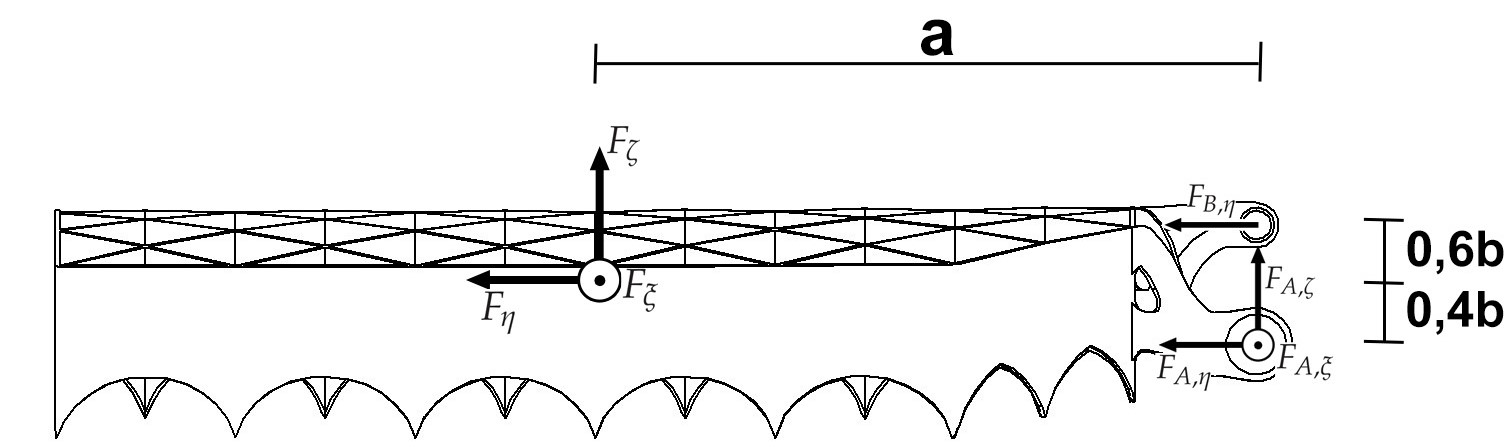
\includegraphics[width=0.6\textwidth]{HaltKraft1.jpg}
	\caption{Halterungskräfte (Seitenansicht)}
	\label{abb_AnhangHK1}
\end{figure}\\
Kräftegleichgewicht in $\zeta$-Richtung:
\begin{equation}\label{eq_h1}
	0 = F_\zeta + F_{A,\zeta}
\end{equation}
Kräftegleichgewicht in $\eta$-Richtung:
\begin{equation}\label{eq_h2}
	0= F_\eta + F_{A,\eta}+F_{B,\eta}
\end{equation}
Momentengleichgewicht in der $\zeta$-$\eta$-Ebene um Halterung A:
\begin{equation}\label{eq_h3}
	0 =F_{B,\eta}b +F_\eta 0,4b  - F_\zeta a
\end{equation}
Mit:
\begin{equation}\label{eq_h4}
	F_{A, \eta} = F_{A1, \eta}+F_{A2, \eta}
\end{equation}
\begin{equation}\label{eq_h5}
	F_{A, \zeta} = F_{A1, \zeta}+F_{A2, \zeta}
\end{equation}
Und aus der Symmetrie folgt:
\begin{equation}\label{eq_h6}
	F_{A1, \zeta}=F_{A2, \zeta} = -\frac{F_\zeta}{2}
\end{equation}
\begin{figure}[h] 
\centering
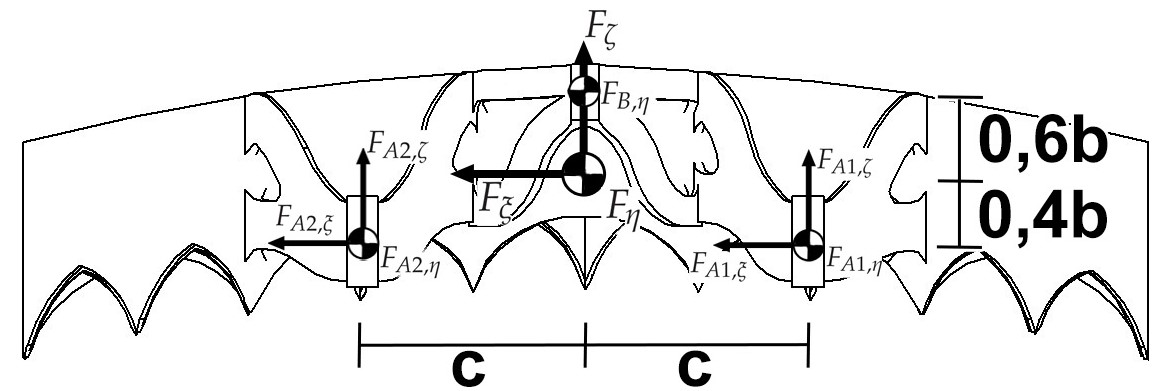
\includegraphics[width=0.6\textwidth]{HaltKraft2.jpg}
\caption{Halterungskräfte (vom Raketenrumpf aus)}
\end{figure}\\
Kräftegleichgewicht in $\xi$-Richtung:
\begin{equation}\label{eq_h7}
	0 = F_\xi + F_{A1,\xi} + F_{A2,\xi}
\end{equation}
Momentengleichgewicht in der $\zeta$-$\xi$-Ebene um Halterung A2:
\begin{equation}\label{eq_h8}
	0= -F_\xi 0.4b - F_{\zeta}c-F_{A1,\zeta}2c
\end{equation}
\begin{figure}[h] 
\centering
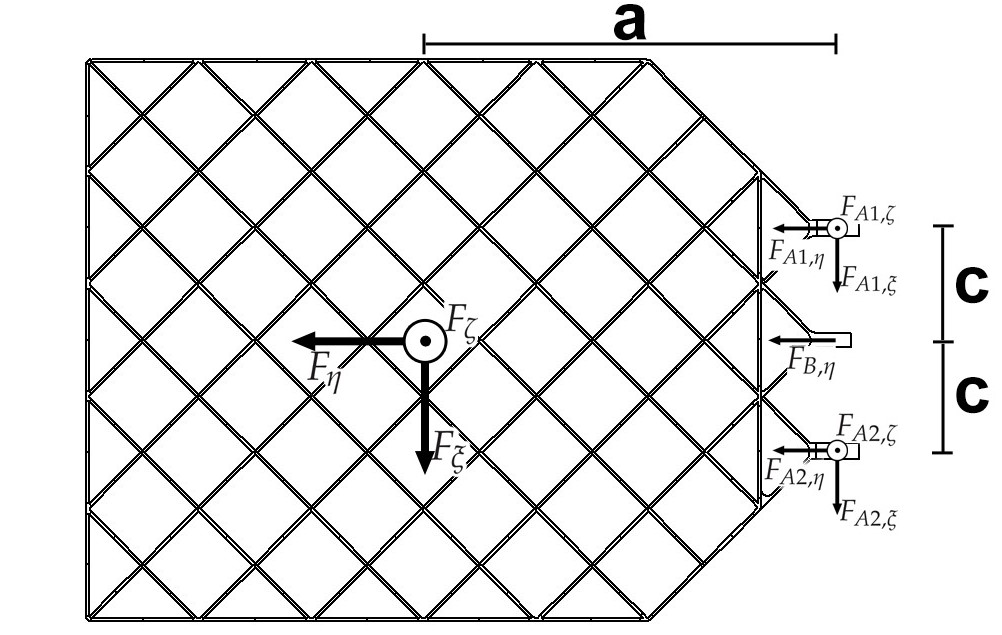
\includegraphics[width=0.6\textwidth]{HaltKraft3.jpg}
\caption{Halterungskräfte (Vorderansicht)}
\label{abb_AnhangHK3}
\end{figure}\\
Momentengleichgewicht in der $\xi$-$\eta$-Ebene um Halterung A2:
\begin{equation}\label{eq_h9}
	0= F_\eta c + F_{\xi}a+F_{b,\eta}c+F_{A1,\eta}2c
\end{equation}
Es ergibt sich aus \ref{eq_h1}:
\begin{equation}\label{eq_h10}
	F_{A, \zeta} = -F_\zeta
\end{equation}
Aus \ref{eq_h3}:
\begin{equation}\label{eq_h11}
	F_{B,\eta} = f_\zeta \frac{a}{b} - F_\eta 0,4
\end{equation}
Aus \ref{eq_h2} und \ref{eq_h11}:
\begin{equation}\label{eq_h12}
	F_{A, \eta} = -F_\zeta \frac{a}{b} - F_\eta 0,6
\end{equation}
Aus \ref{eq_h5}, \ref{eq_h6} und \ref{eq_h10}:
\begin{equation}\label{eq_h13}
	F_{A1, \zeta} = F_{A2, \zeta} = -\frac{F_\zeta}{2}
\end{equation}
Aus \ref{eq_h9} und \ref{eq_h11}:
\begin{equation}\label{eq_h14}
	F_{A1, \zeta} = -\frac{F_\zeta}{4}-F_\xi \frac{a}{2c}-F_\zeta \frac{a}{2b}
\end{equation}
Aus \ref{eq_h4} und \ref{eq_h14}:
\begin{equation}\label{eq_h15}
	F_{A2, \eta} = -\frac{F_\zeta}{4}+F_\xi \frac{a}{2c}-F_\zeta \frac{a}{2b}
\end{equation}
Aus \ref{eq_h7} und \ref{eq_h8}:
\begin{equation}\label{eq_h16}
F_{A1, \xi} = F_{A2, \xi} = -\frac{F_{\xi}}{2}
\end{equation}
Mit $a = 208$ mm, $b=37,5$ mm und $c = 55,6$ mm.
Bisher wurde das Gelenktmoment $M_m$ noch nicht berücksichtigt, sodass sich
\begin{equation}
	F_{A1,\zeta}* = F_{A1,\zeta} +M_m/c
\end{equation}
\begin{equation}
F_{A2,\zeta}* = F_{A2,\zeta} -M_m/c
\end{equation}
 als wirklich vorliegende Kräfte ergibt.